%%%%%%%%%%%%%%%%%%%%%%%%%%%%%%%%%%%%%%%%%
% Class Notes Template
% LaTeX Template
% By: Ryan Grove
%%%%%%%%%%%%%%%%%%%%%%%%%%%%%%%%%%%%%%%%%

%----------------------------------------------------------------------------------------
%	PACKAGES AND OTHER DOCUMENT CONFIGURATIONS
%----------------------------------------------------------------------------------------

\documentclass[paper=a4, fontsize=11pt]{scrartcl} % A4 paper and 11pt font size

\usepackage[T1]{fontenc} % Use 8-bit encoding that has 256 glyphs
\usepackage{fourier} % Use the Adobe Utopia font for the document - comment this line to return to the LaTeX default
\usepackage[english]{babel} % English language/hyphenation
\usepackage{amsmath,amsfonts,amsthm} % Math packages

\usepackage{lipsum} % Used for inserting dummy 'Lorem ipsum' text into the template

\usepackage{sectsty} % Allows customizing section commands
\allsectionsfont{\centering \normalfont\scshape} % Make all sections centered, the default font and small caps

\usepackage{fancyhdr} % Custom headers and footers
\pagestyle{fancyplain} % Makes all pages in the document conform to the custom headers and footers
\fancyhead{} % No page header - if you want one, create it in the same way as the footers below
\fancyfoot[L]{} % Empty left footer
\fancyfoot[C]{} % Empty center footer
%\fancyfoot[R]{\thepage} % Page numbering for right footer
\renewcommand{\headrulewidth}{0pt} % Remove header underlines
\renewcommand{\footrulewidth}{0pt} % Remove footer underlines
\setlength{\headheight}{13.6pt} % Customize the height of the header

\numberwithin{equation}{section} % Number equations within sections (i.e. 1.1, 1.2, 2.1, 2.2 instead of 1, 2, 3, 4)
\numberwithin{figure}{section} % Number figures within sections (i.e. 1.1, 1.2, 2.1, 2.2 instead of 1, 2, 3, 4)
\numberwithin{table}{section} % Number tables within sections (i.e. 1.1, 1.2, 2.1, 2.2 instead of 1, 2, 3, 4)

\setlength\parindent{0pt} % Removes all indentation from paragraphs - comment this line for an assignment with lots of text

\usepackage{lastpage}
\usepackage{fancyhdr}
\cfoot{\thepage\ of \pageref{LastPage}}

\def\v{\hbox{$\mathbf v$}}
\def\w{\hbox{$\mathbf w$}}
\def\u{\hbox{$\mathbf u$}}
\def\x{\hbox{$\textbf{x}$}}
\def\z{\hbox{$\mathbf z$}}
\def\a{\hbox{$\mathbf a$}}
\def\b{\hbox{$\mathbf b$}}
\def\L{\hbox{$\mathcal L$}}
\def\C{\hbox{$\mathbb C$}}
\def\B{\hbox{$\mathcal B$}}
\def\R{\hbox{$\mathbb R$}}
\def\X{\hbox{$\underline X$}}
\def\Q{\hbox{$\mathbb Q$}}
\def\R{\hbox{$\mathbb R$}}
\def\N{\hbox{$\mathbb N$}}
\def\C{\hbox{$\mathbb C$}}
\def\0{\hbox{$\mathbf 0$}}
\def\Y{\hbox{$\underline Y$}}
\def\a{\hbox{$\mathbf a$}}
\def\u{\hbox{$\mathbf u$}}
\def\w{\hbox{$\mathbf w$}}
\def\y{\hbox{$\mathbf y$}}
\def\X{\hbox{$\underline X$}}
\def\dd{\hbox{$\partial $}}
\def\B{\hbox{$\mathcal B$}}
\def\F{\hbox{$\mathcal F$}}
\def\L{\hbox{$\mathcal L$}}
\def\M{\hbox{$\mathcal M$}}
\def\D{\hbox{$\mathscr {D}$}}
\def\RR{\hbox{$\mathscr{R}$}}
\def\I{\hbox{$\mathcal I$}}

\usepackage{amssymb}
%\theoremstyle{plain}
\usepackage[margin = .75in]{geometry}
\newtheorem{claim}{Claim}
\newtheorem{theorem}{Theorem}[section]
\newtheorem{lemma}[theorem]{Lemma}
\newtheorem{proposition}[theorem]{Proposition}
\newtheorem{corollary}[theorem]{Corollary}
\newtheorem{problem}[theorem]{Problem}
%\theoremstyle{definition}
\newtheorem{definition}[theorem]{Definition}
%\theoremstyle{remark}
\newtheorem{remark}[theorem]{Remark}
\newtheorem{remarks}[theorem]{Remarks}
\newtheorem{example}[theorem]{Example}
\newcommand{\ds}{\displaystyle}
\newcommand{\ZZ}{\mathbb{Z}}
\newcommand{\QQ}{\mathbb{Q}}
\newcommand{\e}{\varepsilon}
\newcommand{\bbf}{\textbf}
\newcommand{\p}{\parallel}
\usepackage{color}
\newcommand{\field}[1]{\mathbb{#1}}
\usepackage{amsmath}
\usepackage{amsthm}
\usepackage{amssymb}
\usepackage{mathrsfs}
\usepackage{cancel}
\usepackage{upgreek}
\usepackage{graphicx}
\usepackage{multirow}
\usepackage{setspace}
\usepackage{url}
\usepackage{subfigure}
\usepackage{enumerate}
\usepackage{cases}
\usepackage{mathrsfs}
\usepackage{rotating}

%----------------------------------------------------------------------------------------
%	TITLE SECTION
%----------------------------------------------------------------------------------------

\newcommand{\horrule}[1]{\rule{\linewidth}{#1}} % Create horizontal rule command with 1 argument of height

\title{	
\normalfont \normalsize 
\textsc{Ryan Grove, Clemson University, MATH1080 - 9} \\ [25pt] % Your name, university, class
\horrule{0.5pt} \\[0.4cm] % Thin top horizontal rule
\huge Section 11.4: The Comparison Tests\\ % The assignment title
\horrule{2pt} \\[0.5cm] % Thick bottom horizontal rule
}

\author{Date:} % The due date

\date{\normalsize March 7, 2016} % A custom date

\begin{document}

\maketitle % Print the title

\begin{flushleft}
\begin{tabular}{l l}
Name: \rule{3.2in}{.01cm}  & {}%Table number: \rule{1in}{.01cm}\\
\end{tabular}
\end{flushleft}

%----------------------------------------------------------------------------------------
%	Lecture
%----------------------------------------------------------------------------------------

\section*{\textbf{Lecture:}}
With the comparison tests the idea is to compare a given series with a series that is known to be convergent or divergent.\\
\indent

\fbox{
  \parbox{\textwidth}{
  \vspace{5pt} \textbf{The Comparison Tests}:\\
  \indent
  
   Suppose that $\ds\sum a_n$ and $\ds\sum b_n$ are series with \underline{\hspace{1.25in}} terms.\\
  \indent
  
  \begin{enumerate}
  \item[(i)] If $\ds\sum b_n$ is convergent and $a_n \leq b_n$ for all $n$, then $\ds\sum a_n$ is also \underline{\hspace{1.25in}}.\\
  \item[(ii)] If $\ds\sum b_n$ is divergent and $a_n\geq b_n$ for all $n$, then $\ds\sum a_n $ is also \underline{\hspace{1.25in}}.\\
  \end{enumerate}
  }}
  \indent\\
  \indent
  
  In using the Comparison Test we must have some known series $\ds\sum b_n$ for the purpose of comparison. Most of the time we use one of these series:
  \begin{itemize}
  \item A $p$-series: \quad $\ds\sum\ds\frac{1}{n^p} \text{ }\begin{cases}
  \text{ }\underline{\hspace{1.25in}} & \text{ if } p> 1\\
  \text{ }\underline{\hspace{1.25in}} & \text{ if } p\leq 1
  \end{cases}$\\
  \item A geometric series: \quad $\ds\sum a r^{n-1} \text{ } \begin{cases}
  \text{ } \underline{\hspace{1.25in}} & \text{ if } |r|<1\\
  \text{ } \underline{\hspace{1.25in}} & \text{ if } |r|\geq 1
  \end{cases}$\\
  \end{itemize}
  \indent
  \newpage
  \underline{Example 1}: Determine whether the series $\ds\sum_{n=1}^\infty \ds\frac{5}{2n^2+4n+3}$ converges or diverges.\\
  \indent
  
  
  \vspace{3in}
  
    \[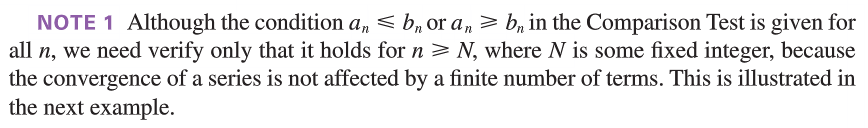
\includegraphics[scale=0.5]{11-4pic1.png}\]
  
  \underline{Example 2}: Test the series $\ds\sum_{k=1}^\infty \ds\frac{\ln k}{k}$ for convergence or divergence.\\
  \indent
  
  \textbf{SOLUTION}: We used the Integral Test to test this series in Example 4 of Section 11.3, but we can also test it by comparing it with the harmonic series.\\
  \indent
  
  \vspace{3.5in}
  
  \[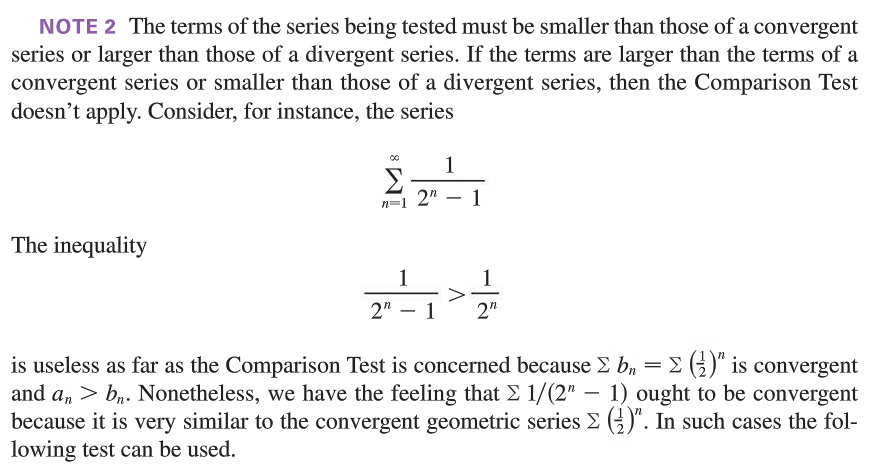
\includegraphics[scale=0.5]{11-4pic2.png}\]
  
  \indent
  
  \fbox{
  \parbox{\textwidth}{
  \vspace{5pt} \textbf{The Limit Comparison Test}: \\
  \indent
  
  Suppose that $\ds\sum a_n$ and $\ds\sum b_n$ are series with positive terms. If
  
  \[\ds\lim_{n\to\infty}\ds\frac{a_n}{b_n} = c\]
  
  where $c$ is a finite number ($c<\infty$) and $c>0$, then either BOTH series \textbf{converge} or BOTH \textbf{diverge}.\\
  }}
  \indent\\
  \indent
  
  (Proof omitted. See page 724 of textbook.)\\
  \indent
  
  \underline{Example 3}: Test the series $\ds\sum_{n=1}^\infty \ds\frac{1}{2^n-1}$ for convergence or divergence.\\
  \indent
  
  \vspace{3in}
  
  \newpage
  
    \textbf{\underline{NOTE}}: We can often find a suitable comparison series $\ds\sum b_n$ by keeping only the highest powers in the numerator and denominator and simplifying the expression.\\
  \indent
  
  \underline{Example 4}: Determine whether the series $\ds\sum_{n=1}^\infty \ds\frac{2n^2+3n}{\ds\sqrt{5+n^5}}$ converges or diverges.\\
  \indent
  
  \vspace{4in}
  

%----------------------------------------------------------------------------------------

\end{document}